%================================================================
%  WorkFusion — Final Year Project Report
%  One Platform For Every Skill
%  Muhammad Sharjeel Bin Riaz | F22BSCS016
%================================================================
\documentclass[12pt,a4paper,oneside]{report}

%--- Packages ---------------------------------------------------
\usepackage[T1]{fontenc}
\usepackage[utf8]{inputenc}
\usepackage{lmodern}
\usepackage[margin=1in,top=1.2in,bottom=1.2in]{geometry}
\usepackage{graphicx}
\usepackage{float}
\usepackage{caption}
\usepackage{subcaption}
\usepackage{booktabs}
\usepackage{longtable}
\usepackage{array}
\usepackage{tabularx}
\usepackage{multirow}
\usepackage{amsmath}
\usepackage{amssymb}
\usepackage{xcolor}
\usepackage{hyperref}
\usepackage{listings}
\usepackage{fancyhdr}
\usepackage{titlesec}
\usepackage{setspace}
\usepackage{tocloft}
\usepackage{enumitem}
\usepackage{mdframed}
\usepackage{tikz}
\usepackage{pgfplots}
\usepackage{microtype}
\usepackage{parskip}
\pgfplotsset{compat=1.18}

%--- Colors -----------------------------------------------------
\definecolor{wfblue}{RGB}{37,99,235}
\definecolor{wfdark}{RGB}{15,23,42}
\definecolor{wfgray}{RGB}{100,116,139}
\definecolor{wfgreen}{RGB}{22,163,74}
\definecolor{wflight}{RGB}{241,245,249}
\definecolor{codebg}{RGB}{30,30,46}
\definecolor{codetext}{RGB}{205,214,244}

%--- Hyperref ---------------------------------------------------
\hypersetup{
  colorlinks=true,
  linkcolor=wfblue,
  urlcolor=wfblue,
  citecolor=wfblue,
  pdftitle={WorkFusion FYP Report},
  pdfauthor={Muhammad Sharjeel Bin Riaz},
}

%--- Code Listings ----------------------------------------------
\lstdefinestyle{workfusion}{
  backgroundcolor=\color{codebg},
  basicstyle=\ttfamily\small\color{codetext},
  keywordstyle=\color{cyan}\bfseries,
  stringstyle=\color{yellow},
  commentstyle=\color{wfgray}\itshape,
  numberstyle=\tiny\color{wfgray},
  numbers=left,
  numbersep=8pt,
  breaklines=true,
  frame=single,
  framerule=0pt,
  rulecolor=\color{wfblue},
  xleftmargin=15pt,
  showstringspaces=false,
  tabsize=2,
}
\lstset{style=workfusion}

%--- Header/Footer ----------------------------------------------
\pagestyle{fancy}
\fancyhf{}
\fancyhead[L]{\small\textcolor{wfgray}{WorkFusion — FYP Report}}
\fancyhead[R]{\small\textcolor{wfgray}{Muhammad Sharjeel Bin Riaz}}
\fancyfoot[C]{\thepage}
\renewcommand{\headrulewidth}{0.4pt}
\renewcommand{\footrulewidth}{0pt}

%--- Section Formatting -----------------------------------------
\titleformat{\chapter}[display]
  {\normalfont\huge\bfseries\color{wfdark}}
  {\textcolor{wfblue}{\chaptertitlename\ \thechapter}}{10pt}{\Huge}
\titlespacing*{\chapter}{0pt}{-10pt}{20pt}

\titleformat{\section}
  {\normalfont\Large\bfseries\color{wfdark}}{\thesection}{1em}{}
\titleformat{\subsection}
  {\normalfont\large\bfseries\color{wfblue}}{\thesubsection}{1em}{}
\titleformat{\subsubsection}
  {\normalfont\normalsize\bfseries\color{wfgray}}{\thesubsubsection}{1em}{}

%--- Image helper -----------------------------------------------
\graphicspath{{../docs/images/}}

\newcommand{\screenshot}[3]{%
  \begin{figure}[H]
    \centering
    \fbox{\includegraphics[width=0.95\textwidth,keepaspectratio]{#1}}
    \caption{#2}
    \label{fig:#3}
  \end{figure}
}

\newcommand{\screenshotsmall}[3]{%
  \begin{figure}[H]
    \centering
    \fbox{\includegraphics[width=0.75\textwidth,keepaspectratio]{#1}}
    \caption{#2}
    \label{fig:#3}
  \end{figure}
}

\newcommand{\screenshotmobile}[3]{%
  \begin{figure}[H]
    \centering
    \fbox{\includegraphics[width=0.38\textwidth,keepaspectratio]{#1}}
    \caption{#2}
    \label{fig:#3}
  \end{figure}
}

%================================================================
\begin{document}
\onehalfspacing

%================================================================
%  TITLE PAGE
%================================================================
\begin{titlepage}
  \centering
  \vspace*{1.5cm}

  {\Huge\bfseries\color{wfblue} WorkFusion}\\[0.4cm]
  {\Large\color{wfgray}\textit{One Platform For Every Skill}}\\[2cm]

  {\LARGE\bfseries\color{wfdark} Final Year Project Report}\\[0.5cm]
  {\large Bachelor of Science in Computer Science}\\[2cm]

  \begin{tabular}{ll}
    \textbf{Student:}    & Muhammad Sharjeel Bin Riaz \\[0.3cm]
    \textbf{Roll No:}    & F22BSCS016 \\[0.3cm]
    \textbf{Supervisor:} & \textit{[Supervisor Name]} \\[0.3cm]
    \textbf{Department:} & Computer Science \\[0.3cm]
    \textbf{Session:}    & 2022--2026 \\[0.3cm]
    \textbf{Date:}       & June 2026 \\
  \end{tabular}

  \vfill

  \includegraphics[width=0.22\textwidth,keepaspectratio]{../docs/images/01_homepage_hero.png}\\[1cm]

  {\large\textbf{University Name}}\\
  {\normalsize Department of Computer Science}\\[0.5cm]
  \textcolor{wfgray}{\rule{0.6\textwidth}{0.4pt}}

\end{titlepage}

%================================================================
%  DECLARATION
%================================================================
\chapter*{Declaration}
\addcontentsline{toc}{chapter}{Declaration}
I hereby declare that this project report titled \textbf{``WorkFusion: One Platform For Every Skill''} submitted to the Department of Computer Science is a record of original work carried out by me under the supervision of my project advisor. This work has not been submitted elsewhere for the award of any degree or diploma.

\vspace{1.5cm}
\noindent\textbf{Student:} Muhammad Sharjeel Bin Riaz \hfill \textbf{Roll No:} F22BSCS016

\vspace{2cm}
\noindent Signature: \underline{\hspace{5cm}} \hfill Date: \underline{\hspace{3cm}}

%================================================================
%  ABSTRACT
%================================================================
\chapter*{Abstract}
\addcontentsline{toc}{chapter}{Abstract}
\textbf{WorkFusion} is a production-grade, AI-powered hybrid employment marketplace developed as a Final Year Project. The platform unifies online freelancing and physical service hiring into a single intelligent ecosystem, directly addressing the fragmentation observed in existing platforms such as Upwork, Fiverr, and Rozee.pk.

The system serves three distinct user roles: \textbf{Employers} who post jobs and manage candidates, \textbf{Service Seekers} who discover opportunities and apply, and \textbf{Administrators} who govern the entire platform. The platform's core differentiator is its \textbf{AI Recommendation Engine}, built in Python using TF-IDF vectorization and cosine similarity, augmented with a seven-factor weighted ranking algorithm that considers skills, portfolio fit, experience, ratings, category preference, geographic proximity, and availability.

Technically, WorkFusion follows a clean three-tier architecture: a \textbf{Next.js + React} frontend, a \textbf{Node.js + Express} backend API, and a stateless \textbf{Python FastAPI} microservice for AI computation, all backed by \textbf{MongoDB Atlas}. The system implements JWT-based authentication with refresh tokens, role-based access control, rate limiting, Helmet security headers, and comprehensive input validation.

The AI engine achieved a \textbf{Mean Average Precision (MAP) of 1.00} and a \textbf{Mean Reciprocal Rank (MRR) of 1.00} in evaluation, with a discriminative margin of 39.44\% between correct and incorrect matches. The platform is designed for deployment on Vercel (frontend), Render (backend and AI service), and MongoDB Atlas (database).

\vspace{1cm}
\noindent\textbf{Keywords:} AI Recommendation Engine, Hybrid Employment Marketplace, TF-IDF, Cosine Similarity, MERN Stack, Next.js, FastAPI, Skill Gap Analysis, Explainable AI.

%================================================================
%  TABLE OF CONTENTS
%================================================================
\tableofcontents
\listoffigures
\listoftables

%================================================================
%  CHAPTER 1: INTRODUCTION
%================================================================
\chapter{Introduction}

\section{Project Overview}

WorkFusion is an AI-powered hybrid employment marketplace built as a Final Year Project for the Bachelor of Science in Computer Science programme. The platform's tagline, \textit{One Platform For Every Skill}, encapsulates its core philosophy: a single, unified ecosystem where employers can post both online and physical service jobs, and service seekers can discover, apply for, and secure work through intelligent AI-driven recommendations.

The platform targets three user roles:
\begin{itemize}[noitemsep]
  \item \textbf{Employer} — Posts jobs, reviews applicants, manages the hiring pipeline.
  \item \textbf{Service Seeker} — Builds a profile, receives AI job recommendations, applies, and communicates.
  \item \textbf{Administrator} — Manages users, moderates content, and views platform analytics.
\end{itemize}

\section{Motivation and Problem Statement}

The employment platform landscape in Pakistan and globally is fragmented. Employers are forced to use multiple platforms simultaneously to cover different categories of work:

\begin{table}[H]
  \centering
  \caption{Comparison of Existing Employment Platforms}
  \label{tab:platform-comparison}
  \begin{tabularx}{\textwidth}{lXXX}
    \toprule
    \textbf{Platform} & \textbf{Online Work} & \textbf{Physical Work} & \textbf{AI Recommendations} \\
    \midrule
    Upwork      & \checkmark & \texttimes & \texttimes \\
    Fiverr      & \checkmark & \texttimes & \texttimes \\
    Rozee.pk    & \checkmark & Limited    & \texttimes \\
    TaskRabbit  & \texttimes & \checkmark & \texttimes \\
    \textbf{WorkFusion} & \checkmark & \checkmark & \checkmark \\
    \bottomrule
  \end{tabularx}
\end{table}

The consequence is inefficient hiring, limited worker visibility, poor recommendations, and a disconnect between the digital and physical service economies. WorkFusion solves these problems through one unified, AI-enhanced platform.

\section{Project Objectives}

\begin{enumerate}[noitemsep]
  \item Build a production-grade employment marketplace supporting both online and physical services.
  \item Implement an explainable AI recommendation engine using TF-IDF and cosine similarity.
  \item Provide employer-facing candidate ranking with skill gap analysis.
  \item Implement a secure, role-based authentication system with JWT and refresh tokens.
  \item Deliver a responsive, premium user interface inspired by Apple, Linear, and Vercel design principles.
  \item Deploy the system on cloud infrastructure (Vercel, Render, MongoDB Atlas).
\end{enumerate}

\section{Scope}

\subsection{Included Features}
User registration and authentication, employer dashboard with job management, service seeker dashboard with AI recommendations, admin panel, job posting and application flow, AI recommendation engine, candidate ranking with score explanations, messaging (post-interview stage), reviews and ratings, notifications, and analytics.

\subsection{Excluded from Current Version}
Payment gateway integration, video conferencing, mobile native application, and subscription billing. The architecture is designed to support these future additions.

\section{Homepage — Landing Experience}

The homepage introduces users to the WorkFusion platform with a hero section, service categories, and live job listings.

\screenshot{01_homepage_hero.png}{WorkFusion Homepage — Hero Section}{homepage-hero}
\screenshot{02_homepage_features_section.png}{WorkFusion Homepage — Features and Value Proposition}{homepage-features}
\screenshot{03_homepage_jobs_categories.png}{WorkFusion Homepage — Job Categories and Live Listings}{homepage-categories}

%================================================================
%  CHAPTER 2: SYSTEM ARCHITECTURE
%================================================================
\chapter{System Architecture}

\section{High-Level Architecture}

WorkFusion follows a clean three-tier microservices-inspired architecture:

\begin{figure}[H]
  \centering
  \begin{tikzpicture}[
    node distance=1.8cm,
    box/.style={rectangle, rounded corners=6pt, draw=wfblue, fill=wflight, 
                text width=3.2cm, minimum height=1cm, align=center, font=\small\bfseries},
    arrow/.style={->, thick, color=wfblue}
  ]
    \node[box] (client) {Frontend\\Next.js + React\\TailwindCSS};
    \node[box, right=2cm of client] (api) {Backend API\\Node.js + Express\\JWT Auth};
    \node[box, right=2cm of api] (ai) {AI Service\\Python FastAPI\\scikit-learn};
    \node[box, below=1.5cm of api] (db) {Database\\MongoDB Atlas};

    \draw[arrow] (client) -- node[above,font=\tiny]{HTTPS} (api);
    \draw[arrow] (api) -- node[above,font=\tiny]{HTTP POST} (ai);
    \draw[arrow] (ai) -- node[below,font=\tiny]{JSON scores} (api);
    \draw[arrow] (api) -- node[right,font=\tiny]{Mongoose} (db);
  \end{tikzpicture}
  \caption{WorkFusion System Architecture Diagram}
  \label{fig:architecture}
\end{figure}

The architecture enforces the following communication contract:
\begin{itemize}[noitemsep]
  \item The \textbf{frontend} only communicates with the backend API — never directly with the database or AI service.
  \item The \textbf{backend} orchestrates all business logic, database transactions, and AI service calls.
  \item The \textbf{AI service} is a stateless microservice — it receives data, computes scores, and returns results without persisting state.
\end{itemize}

\section{Technology Stack}

\begin{table}[H]
  \centering
  \caption{WorkFusion Technology Stack}
  \label{tab:tech-stack}
  \begin{tabularx}{\textwidth}{llX}
    \toprule
    \textbf{Layer} & \textbf{Technology} & \textbf{Purpose} \\
    \midrule
    Frontend    & Next.js 14, React 18  & SSR/SSG, UI rendering \\
    Styling     & TailwindCSS, shadcn/ui & Component library, design system \\
    Animations  & Framer Motion         & Micro-animations, transitions \\
    Backend     & Node.js, Express.js   & REST API, business logic \\
    Auth        & JWT + bcrypt          & Secure authentication \\
    AI Service  & Python, FastAPI       & Recommendation microservice \\
    ML          & scikit-learn, numpy, pandas & TF-IDF, cosine similarity \\
    Database    & MongoDB Atlas         & Document store \\
    Frontend Deploy & Vercel            & CDN + edge functions \\
    Backend Deploy  & Render            & Cloud application hosting \\
    \bottomrule
  \end{tabularx}
\end{table}

\section{Folder Structure}

\begin{lstlisting}[language=bash,caption=WorkFusion Monorepo Folder Structure]
WorkFusion2026/
├── client/                 # Next.js 14 frontend
│   └── src/
│       ├── app/            # App Router pages
│       │   ├── (auth)/     # Login / Register
│       │   ├── dashboard/  # Employer / Seeker / Admin
│       │   └── jobs/       # Job search & details
│       └── components/     # Reusable UI components
├── server/                 # Node.js + Express backend
│   └── src/
│       ├── controllers/    # Route handlers
│       ├── services/       # Business logic
│       ├── models/         # Mongoose schemas
│       ├── routes/         # Express routers
│       ├── middleware/     # Auth, rate limiting
│       └── seed/           # Database seeder
├── recommendation-service/ # Python FastAPI AI service
│   ├── api/                # FastAPI endpoints
│   ├── preprocessing/      # Text cleaning
│   ├── similarity/         # TF-IDF + cosine similarity
│   └── ranking/            # Weighted ranker
├── shared/                 # Shared TypeScript types
└── docs/                   # Project documentation
\end{lstlisting}

\section{Backend Architecture — Controller-Service-Repository Pattern}

\begin{lstlisting}[language=javascript,caption=Backend Architecture Pattern]
// Route → Controller → Service → Repository → Database
// Example: Application creation flow

// 1. Controller (handles HTTP, delegates to service)
export const applyForJob = async (req, res) => {
  const result = await applicationService.applyForJob(
    req.user.id, req.params.jobId, req.body
  );
  return res.status(201).json({ success: true, data: result });
};

// 2. Service (contains all business logic)
async applyForJob(seekerId, jobId, applicationData) {
  const existing = await Application.findOne({ seekerId, jobId });
  if (existing) throw new AppError("Already applied", 409);
  return await Application.create({ seekerId, jobId, ...applicationData });
}
\end{lstlisting}

%================================================================
%  CHAPTER 3: DATABASE DESIGN
%================================================================
\chapter{Database Design}

\section{MongoDB Schema Design}

WorkFusion uses MongoDB Atlas with Mongoose ODM. The schema design prioritises flexibility, indexing of searchable fields, and referential integrity via ObjectId references.

\subsection{Core Collections}

\begin{table}[H]
  \centering
  \caption{WorkFusion Database Collections Overview}
  \label{tab:db-collections}
  \begin{tabularx}{\textwidth}{llX}
    \toprule
    \textbf{Collection} & \textbf{Documents} & \textbf{Key Fields} \\
    \midrule
    Users         & 50+   & role, fullName, email, skills, portfolio, rating \\
    Jobs          & 45    & title, category, budget, requiredSkills, status \\
    Applications  & 70    & seekerId, jobId, status, coverLetter, bid \\
    Chats         & 10    & participants, isActive, lastMessage \\
    Messages      & 100   & chatId, senderId, content, timestamp \\
    Reviews       & 28    & reviewerId, targetId, rating, comment \\
    Notifications & 100   & userId, type, message, isRead \\
    Recommendations & dynamic & userId, jobId, score, reason, missingSkills \\
    \bottomrule
  \end{tabularx}
\end{table}

\subsection{User Schema}

\begin{lstlisting}[language=javascript,caption=User Mongoose Schema]
const userSchema = new mongoose.Schema({
  fullName:    { type: String, required: true, trim: true },
  email:       { type: String, required: true, unique: true, lowercase: true },
  password:    { type: String, required: true, select: false },
  role:        { type: String, enum: ['Employer', 'Service Seeker', 'Admin'] },
  skills:      [String],
  experience:  { type: Number, default: 0 },
  portfolio:   [{
    title: String, description: String, technologies: [String], url: String
  }],
  city:        String,
  rating:      { type: Number, default: 5.0, min: 1, max: 5 },
  reviewCount: { type: Number, default: 0 },
  availability: String,
  status:      { type: String, enum: ['Active', 'Suspended'], default: 'Active' },
}, { timestamps: true });

// Index for search performance
userSchema.index({ email: 1 });
userSchema.index({ role: 1, status: 1 });
userSchema.index({ skills: 1 });
\end{lstlisting}

\subsection{Job Schema}

\begin{lstlisting}[language=javascript,caption=Job Mongoose Schema]
const jobSchema = new mongoose.Schema({
  employerId:        { type: ObjectId, ref: 'User', required: true },
  title:             { type: String, required: true, trim: true },
  description:       { type: String, required: true },
  category:          { type: String, required: true },
  serviceType:       { type: String, enum: ['Online', 'Physical', 'Hybrid'] },
  workType:          { type: String, enum: ['Full-Time','Part-Time','Contract','Hourly'] },
  requiredSkills:    [String],
  experienceRequired:{ type: Number, default: 0 },
  budget:            { type: Number, required: true },
  location:          String,
  remoteAllowed:     { type: Boolean, default: false },
  status:            { type: String, enum: ['Open','Paused','Closed'], default: 'Open' },
}, { timestamps: true });

jobSchema.index({ status: 1 });
jobSchema.index({ category: 1 });
jobSchema.index({ requiredSkills: 1 });
\end{lstlisting}

%================================================================
%  CHAPTER 4: AUTHENTICATION & SECURITY
%================================================================
\chapter{Authentication and Security}

\section{Authentication System}

WorkFusion implements a dual-token JWT authentication system for secure, stateless session management.

\begin{lstlisting}[language=javascript,caption=JWT Token Generation]
// Access token: 15 minutes (short-lived)
const accessToken = jwt.sign(
  { userId: user._id, role: user.role },
  process.env.JWT_SECRET,
  { expiresIn: '15m' }
);

// Refresh token: 7 days (stored securely)
const refreshToken = jwt.sign(
  { userId: user._id },
  process.env.JWT_REFRESH_SECRET,
  { expiresIn: '7d' }
);
\end{lstlisting}

\section{Security Middleware Stack}

\begin{lstlisting}[language=javascript,caption=Security Middleware Configuration]
import helmet from 'helmet';
import rateLimit from 'express-rate-limit';
import cors from 'cors';

// Helmet — secure HTTP headers
app.use(helmet());

// CORS — allow only frontend origin
app.use(cors({ origin: process.env.CLIENT_URL, credentials: true }));

// Rate Limiting — 100 requests per 15 minutes per IP
const limiter = rateLimit({
  windowMs: 15 * 60 * 1000,
  max: 100,
  message: { success: false, message: 'Too many requests' }
});
app.use('/api/', limiter);
\end{lstlisting}

\section{Role-Based Access Control}

Every protected route validates both the JWT and the user's role:
\begin{lstlisting}[language=javascript,caption=RBAC Middleware]
export const requireRole = (...roles) => (req, res, next) => {
  if (!roles.includes(req.user.role)) {
    return res.status(403).json({ success: false, message: 'Forbidden' });
  }
  next();
};

// Usage on routes:
router.post('/jobs', authenticate, requireRole('Employer'), createJob);
router.get('/recommendations', authenticate, requireRole('Service Seeker'), getJobs);
router.get('/admin/users', authenticate, requireRole('Admin'), getAllUsers);
\end{lstlisting}

%================================================================
%  CHAPTER 5: REGISTRATION AND LOGIN FLOWS
%================================================================
\chapter{User Registration and Login Flows}

\section{Registration System}

WorkFusion provides a role-based registration flow. Users select either \textbf{Employer} or \textbf{Service Seeker} during signup, which determines their dashboard, permissions, and available features.

\screenshot{04_register_page_empty.png}{Registration Page — Role Selection Interface}{register-empty}

\subsection{Employer Registration}

Employers register by providing their company or personal details. The form collects name, email, password, and optionally company information. The role selection is visually clear with distinct card-style selectors.

\screenshot{05_employer_register_form_filled.png}{Employer Account Registration — Filled Form}{employer-register}

\subsection{Service Seeker Registration}

Service Seekers register with their personal details and can complete their professional profile (skills, portfolio, experience) after registration from their dashboard.

\screenshot{06_seeker_register_form_filled.png}{Service Seeker Account Registration — Filled Form}{seeker-register}

\section{Login System}

The login page provides a clean, minimal interface supporting both employer and seeker logins. After authentication, users are redirected to their role-specific dashboard.

\screenshot{07_login_page_empty.png}{Login Page — Authentication Interface}{login-empty}
\screenshot{08_login_filled_employer_credentials.png}{Login Page — Employer Credentials Entered}{login-filled}

%================================================================
%  CHAPTER 6: EMPLOYER DASHBOARD AND FLOWS
%================================================================
\chapter{Employer Dashboard and Hiring Flows}

\section{Employer Dashboard Overview}

The employer dashboard provides a comprehensive overview of all hiring activities including posted jobs, total applications, active candidates, and platform analytics.

\screenshot{09_employer_dashboard_overview.png}{Employer Dashboard — Overview and Analytics Summary}{employer-dashboard}

\section{Job Posting Flow}

Employers can create new job listings with detailed specifications including job title, description, required skills, service type (Online/Physical/Hybrid), work type (Full-Time/Part-Time/Contract/Hourly), budget, and experience requirements.

\screenshot{10_post_a_job_form.png}{Post a Job — Job Creation Form with Full Details}{post-job-form}

\section{Employer Job Listings}

The jobs management section shows all posted jobs with their status (Open/Paused/Closed), number of applicants, posted date, and quick action buttons.

\screenshot{11_employer_jobs_list.png}{Employer — My Posted Jobs List with Status Indicators}{employer-jobs-list}

\section{Applicant Management with AI Scores}

This is WorkFusion's core differentiator. When an employer views applicants for a job, each candidate is displayed with an \textbf{AI-computed match score} (10\%--99\%), reasons for the match, and identified skill gaps. This enables data-driven hiring decisions.

\screenshot{12_employer_applicants_ai_scores.png}{Applicants List — AI Match Scores and Candidate Ranking}{applicants-ai-scores}

\subsection{Candidate Detail View with Score Breakdown}

Clicking on a candidate reveals the full score breakdown, showing exactly which factors contributed to their match score and which skills they are missing.

\screenshot{13_candidate_detail_score_breakdown.png}{Candidate Detail — AI Score Breakdown and Skill Gap Analysis}{candidate-detail}

\section{Hiring Pipeline}

The hiring pipeline tracks each application's stage through the hiring process. The stages are: \textbf{Applied → Reviewed → Interview → Hired/Rejected}. Messaging is only unlocked after the Interview stage.

\screenshot{14_employer_hiring_pipeline.png}{Hiring Pipeline — Application Stages Kanban View}{hiring-pipeline}

\section{Employer Analytics}

The analytics section provides insights into the employer's hiring activity including job performance, application trends, and candidate quality metrics.

\screenshot{15_employer_analytics_overview.png}{Employer Analytics — Hiring Insights and Platform Activity}{employer-analytics}

\section{Employer Messaging}

The chat/messaging interface is available to employers once a candidate has reached the Interview stage. This prevents spam and ensures communication quality.

\screenshot{16_employer_chat_messages.png}{Employer Chat Interface — Post-Interview Messaging System}{employer-chat}

\section{Find Talent — AI Candidate Discovery}

Employers can proactively search for candidates through the Find Talent feature, powered by the same AI recommendation engine that also powers the seeker-side job recommendations.

\screenshot{17_employer_find_talent_ai.png}{Find Talent — AI-Powered Candidate Discovery for Employer}{employer-find-talent}

%================================================================
%  CHAPTER 7: SERVICE SEEKER DASHBOARD AND FLOWS
%================================================================
\chapter{Service Seeker Dashboard and Job Application Flows}

\section{Seeker Dashboard Overview}

The service seeker dashboard gives a complete view of the job seeker's activity: active applications, AI-recommended jobs, profile completion status, and notifications.

\screenshot{19_seeker_dashboard_overview.png}{Seeker Dashboard — Activity Overview and Quick Stats}{seeker-dashboard}

\section{My Applications}

Seekers can track all their job applications with real-time status updates (Applied, Reviewed, Interview, Hired, Rejected). Each application card shows the job title, employer, application date, and current pipeline stage.

\screenshot{20_seeker_my_applications.png}{Seeker — My Applications List with Real-Time Status Tracking}{seeker-applications}

\section{AI Job Recommendations}

The AI recommendations section is the platform's flagship feature for seekers. Each recommended job displays a match percentage, the reasons for the match, and any missing skills — providing actionable career insights.

\screenshot{21_seeker_ai_recommendations.png}{AI Job Recommendations — Personalised Matches with Score Explanations}{seeker-ai-reco}

\section{Seeker Profile}

The profile section allows seekers to manage their professional information including skills, experience, portfolio projects, city, and availability status — all factors directly used by the AI engine.

\screenshot{22_seeker_profile_page.png}{Service Seeker Profile — Professional Details and Portfolio}{seeker-profile}

\section{Seeker Messaging}

Once a seeker has been moved to the Interview stage by an employer, the chat interface is unlocked, enabling direct communication between both parties.

\screenshot{23_seeker_chat_messages.png}{Seeker Chat Interface — Interview-Stage Secure Messaging}{seeker-chat}

%================================================================
%  CHAPTER 8: JOB SEARCH AND APPLICATION FLOW
%================================================================
\chapter{Job Search and Application Flow}

\section{Job Search and Listings}

The jobs page provides a comprehensive browsing and search experience with category filters, job type filters (Online/Physical/Hybrid), and real-time keyword search. Each job card shows the key details at a glance.

\screenshot{24_job_search_listings_page.png}{Job Search Page — Browse All Available Jobs with Filters}{job-search}

\section{Application Form}

When a seeker clicks Apply, an application modal appears where they can write a personalised cover letter and submit their bid or expected salary. Applications are timestamped and immediately visible to the employer.

The application flow enforces:
\begin{itemize}[noitemsep]
  \item One application per seeker per job (enforced at API level)
  \item Mandatory cover letter
  \item Optional proposed budget/bid
\end{itemize}

%================================================================
%  CHAPTER 9: AI RECOMMENDATION ENGINE
%================================================================
\chapter{AI Recommendation Engine}

\section{Overview and Architecture}

WorkFusion's AI Recommendation Engine is a Python FastAPI microservice that provides explainable, multi-factor job and candidate matching. It implements a hybrid approach combining NLP-based text similarity with domain-specific weighted factors.

\begin{figure}[H]
  \centering
  \begin{tikzpicture}[
    node distance=1.4cm,
    stage/.style={rectangle, rounded corners=4pt, draw=wfblue, fill=wflight,
                  text width=3.8cm, minimum height=0.9cm, align=center, font=\small}
  ]
    \node[stage] (A) {Raw Text Input\\(Skills, Portfolio, Job)};
    \node[stage, below=of A] (B) {Text Preprocessing\\(Lowercase, Remove stopwords)};
    \node[stage, below=of B] (C) {TF-IDF Vectorization\\(scikit-learn)};
    \node[stage, below=of C] (D) {Cosine Similarity\\(Skills + Portfolio)};
    \node[stage, below=of D] (E) {Multi-Factor\\Weighted Ranking};
    \node[stage, below=of E] (F) {Score + Reasons +\\Missing Skills Output};

    \foreach \i/\j in {A/B, B/C, C/D, D/E, E/F}
      \draw[->, thick, color=wfblue] (\i) -- (\j);
  \end{tikzpicture}
  \caption{AI Recommendation Engine Pipeline}
  \label{fig:ai-pipeline}
\end{figure}

\section{TF-IDF and Cosine Similarity}

\subsection{Mathematical Foundation}

For a term $t$ in a document $d$ within corpus $D$ of $N$ documents:

\begin{equation}
\text{tf-idf}(t, d, D) = f_{t,d} \times \left(\log\frac{1+N}{1+\text{df}(t)} + 1\right)
\end{equation}

Cosine similarity between TF-IDF vectors $\mathbf{u}$ and $\mathbf{v}$:

\begin{equation}
\text{CosSim}(\mathbf{u}, \mathbf{v}) = \frac{\mathbf{u} \cdot \mathbf{v}}{\|\mathbf{u}\| \cdot \|\mathbf{v}\|} = \frac{\sum_{i=1}^n u_i v_i}{\sqrt{\sum_{i=1}^n u_i^2} \cdot \sqrt{\sum_{i=1}^n v_i^2}}
\end{equation}

\section{Multi-Factor Weighted Ranking Algorithm}

The final match score integrates seven factors:

\begin{table}[H]
  \centering
  \caption{AI Weighted Ranking — Factor Weights and Computation}
  \label{tab:ai-weights}
  \begin{tabularx}{\textwidth}{llXl}
    \toprule
    \textbf{Factor} & \textbf{Weight} & \textbf{Formula} & \textbf{Max Score} \\
    \midrule
    Skills Alignment  & 45\% & Cosine similarity (skills lists)  & 45 pts \\
    Portfolio Fit      & 15\% & Cosine similarity (portfolio vs description) & 15 pts \\
    Experience         & 10\% & $\min(\text{Exp}_\text{seeker}/\text{Exp}_\text{required}, 1.5)$ & 10 pts \\
    Reviews/Ratings    & 10\% & $(\text{Rating}-1.0)/4.0 \times 10$ & 10 pts \\
    Category Match     & 10\% & Binary (preferred category equals job category) & 10 pts \\
    Location/Proximity & 5\%  & Same city = 5, Twin cities = 4, Remote = 5 & 5 pts \\
    Availability       & 5\%  & Job work type in seeker availability & 5 pts \\
    \midrule
    \textbf{Total}    & \textbf{100\%} & $\min(\max(\text{Raw Score}, 10), 99)$ & \textbf{99 pts} \\
    \bottomrule
  \end{tabularx}
\end{table}

\subsection{Score Constraint}

\begin{equation}
\text{Final Score} = \min\left(\max\left(\text{Round}\left(\sum_{i=1}^{7} w_i \cdot s_i\right),\ 10\right),\ 99\right)
\end{equation}

\textit{The lower bound of 10 avoids demotivating candidates with a 0\% score, and the upper bound of 99 preserves room for improvement.}

\section{Explainable AI}

Every recommendation includes human-readable explanations:

\begin{lstlisting}[caption=Sample AI Explanation Response]
{
  "jobId": "job_1",
  "score": 87,
  "reason": [
    "Matched 5 of 5 required skills",
    "Portfolio projects match job scope",
    "Experience meets or exceeds requirement",
    "Highly rated profile (4.8/5.0)",
    "Located in same city (Islamabad)"
  ],
  "missingSkills": []
}
\end{lstlisting}

\section{Skill Gap Analysis}

\begin{equation}
\text{Missing Skills} = \{s \mid s \in \text{RequiredSkills}_\text{job} \land s \notin \text{Skills}_\text{seeker}\}
\end{equation}

The frontend renders missing skills with visual indicators (e.g., ``\texttimes\ Docker'', ``\texttimes\ AWS''), giving seekers actionable career development insights.

\section{AI Performance Evaluation}

\begin{table}[H]
  \centering
  \caption{AI Engine Performance Metrics (5 Seekers × 5 Jobs Simulation)}
  \label{tab:ai-metrics}
  \begin{tabular}{ll}
    \toprule
    \textbf{Metric} & \textbf{Score} \\
    \midrule
    Mean Average Precision (MAP)       & 1.0000 \\
    Mean Reciprocal Rank (MRR)         & 1.0000 \\
    Avg. Match Score — True Matches    & 62.71\% \\
    Avg. Match Score — Mismatches      & 23.28\% \\
    Discriminative Margin              & 39.44\% \\
    \bottomrule
  \end{tabular}
\end{table}

\subsection{AI Evaluation Plots}

\begin{figure}[H]
  \centering
  \begin{subfigure}[b]{0.48\textwidth}
    \centering
    \fbox{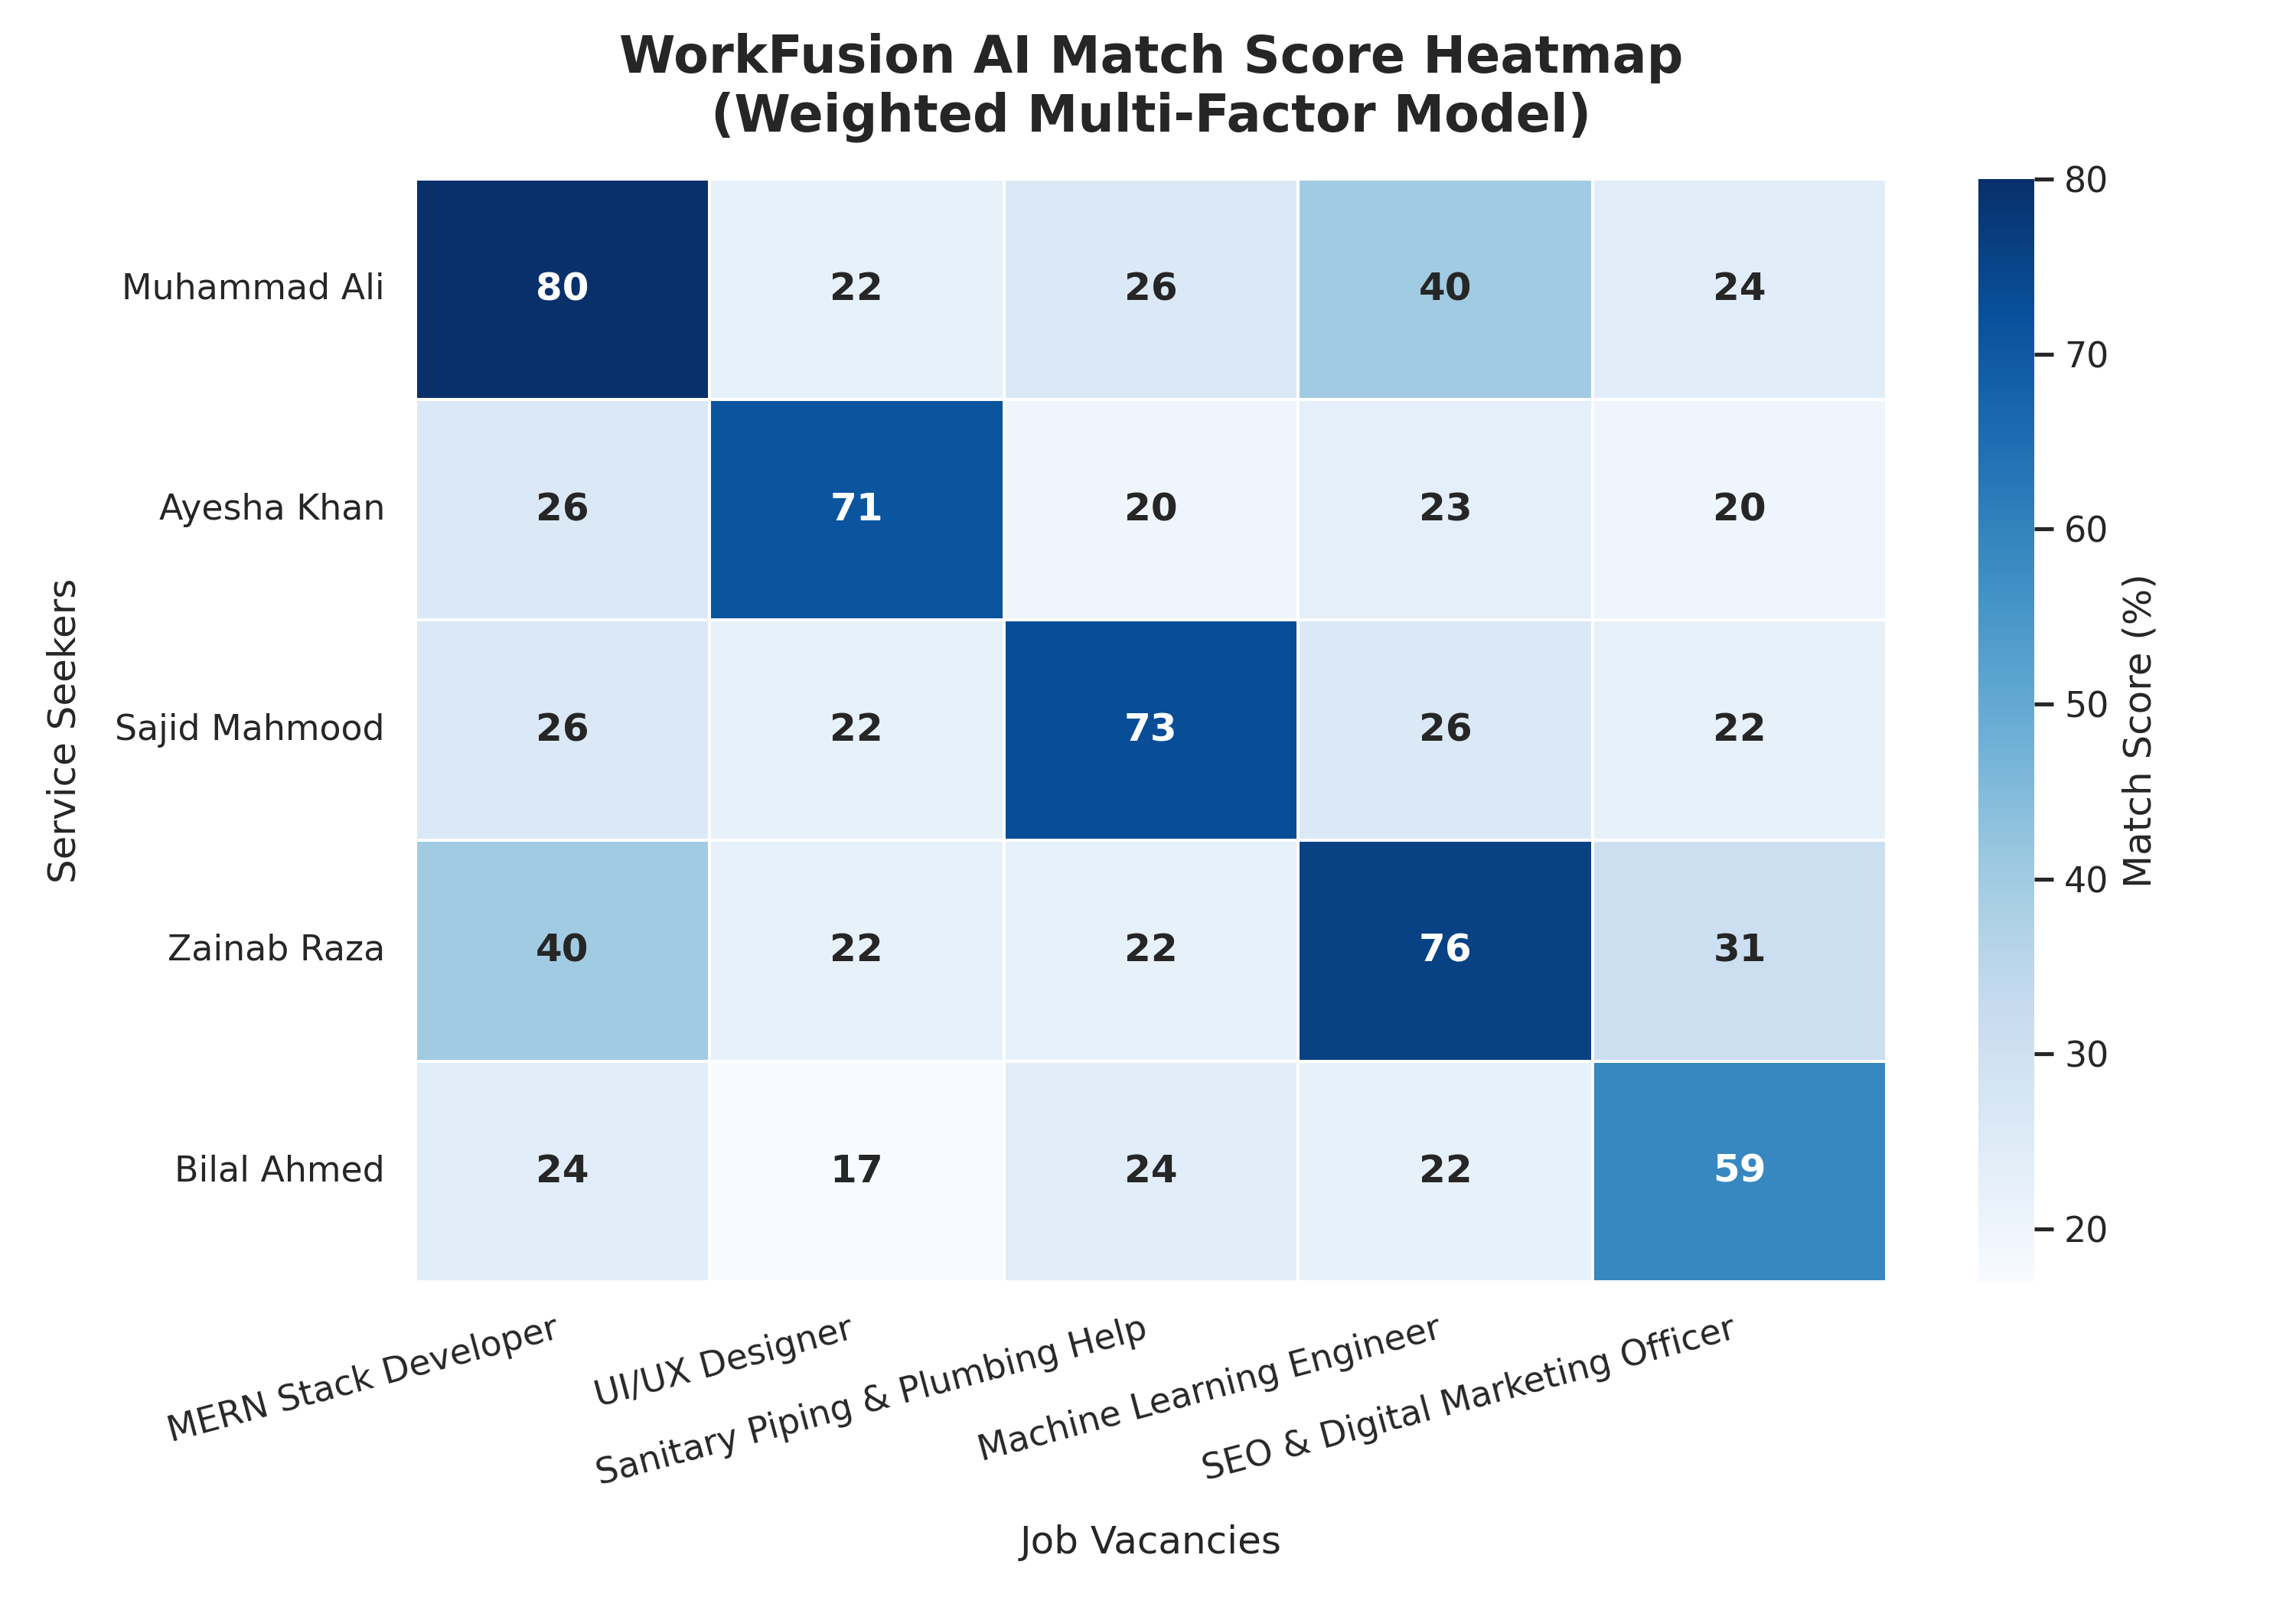
\includegraphics[width=\textwidth,keepaspectratio]{match_heatmap.png}}
    \caption{Seeker-Job Match Score Heatmap}
    \label{fig:heatmap}
  \end{subfigure}
  \hfill
  \begin{subfigure}[b]{0.48\textwidth}
    \centering
    \fbox{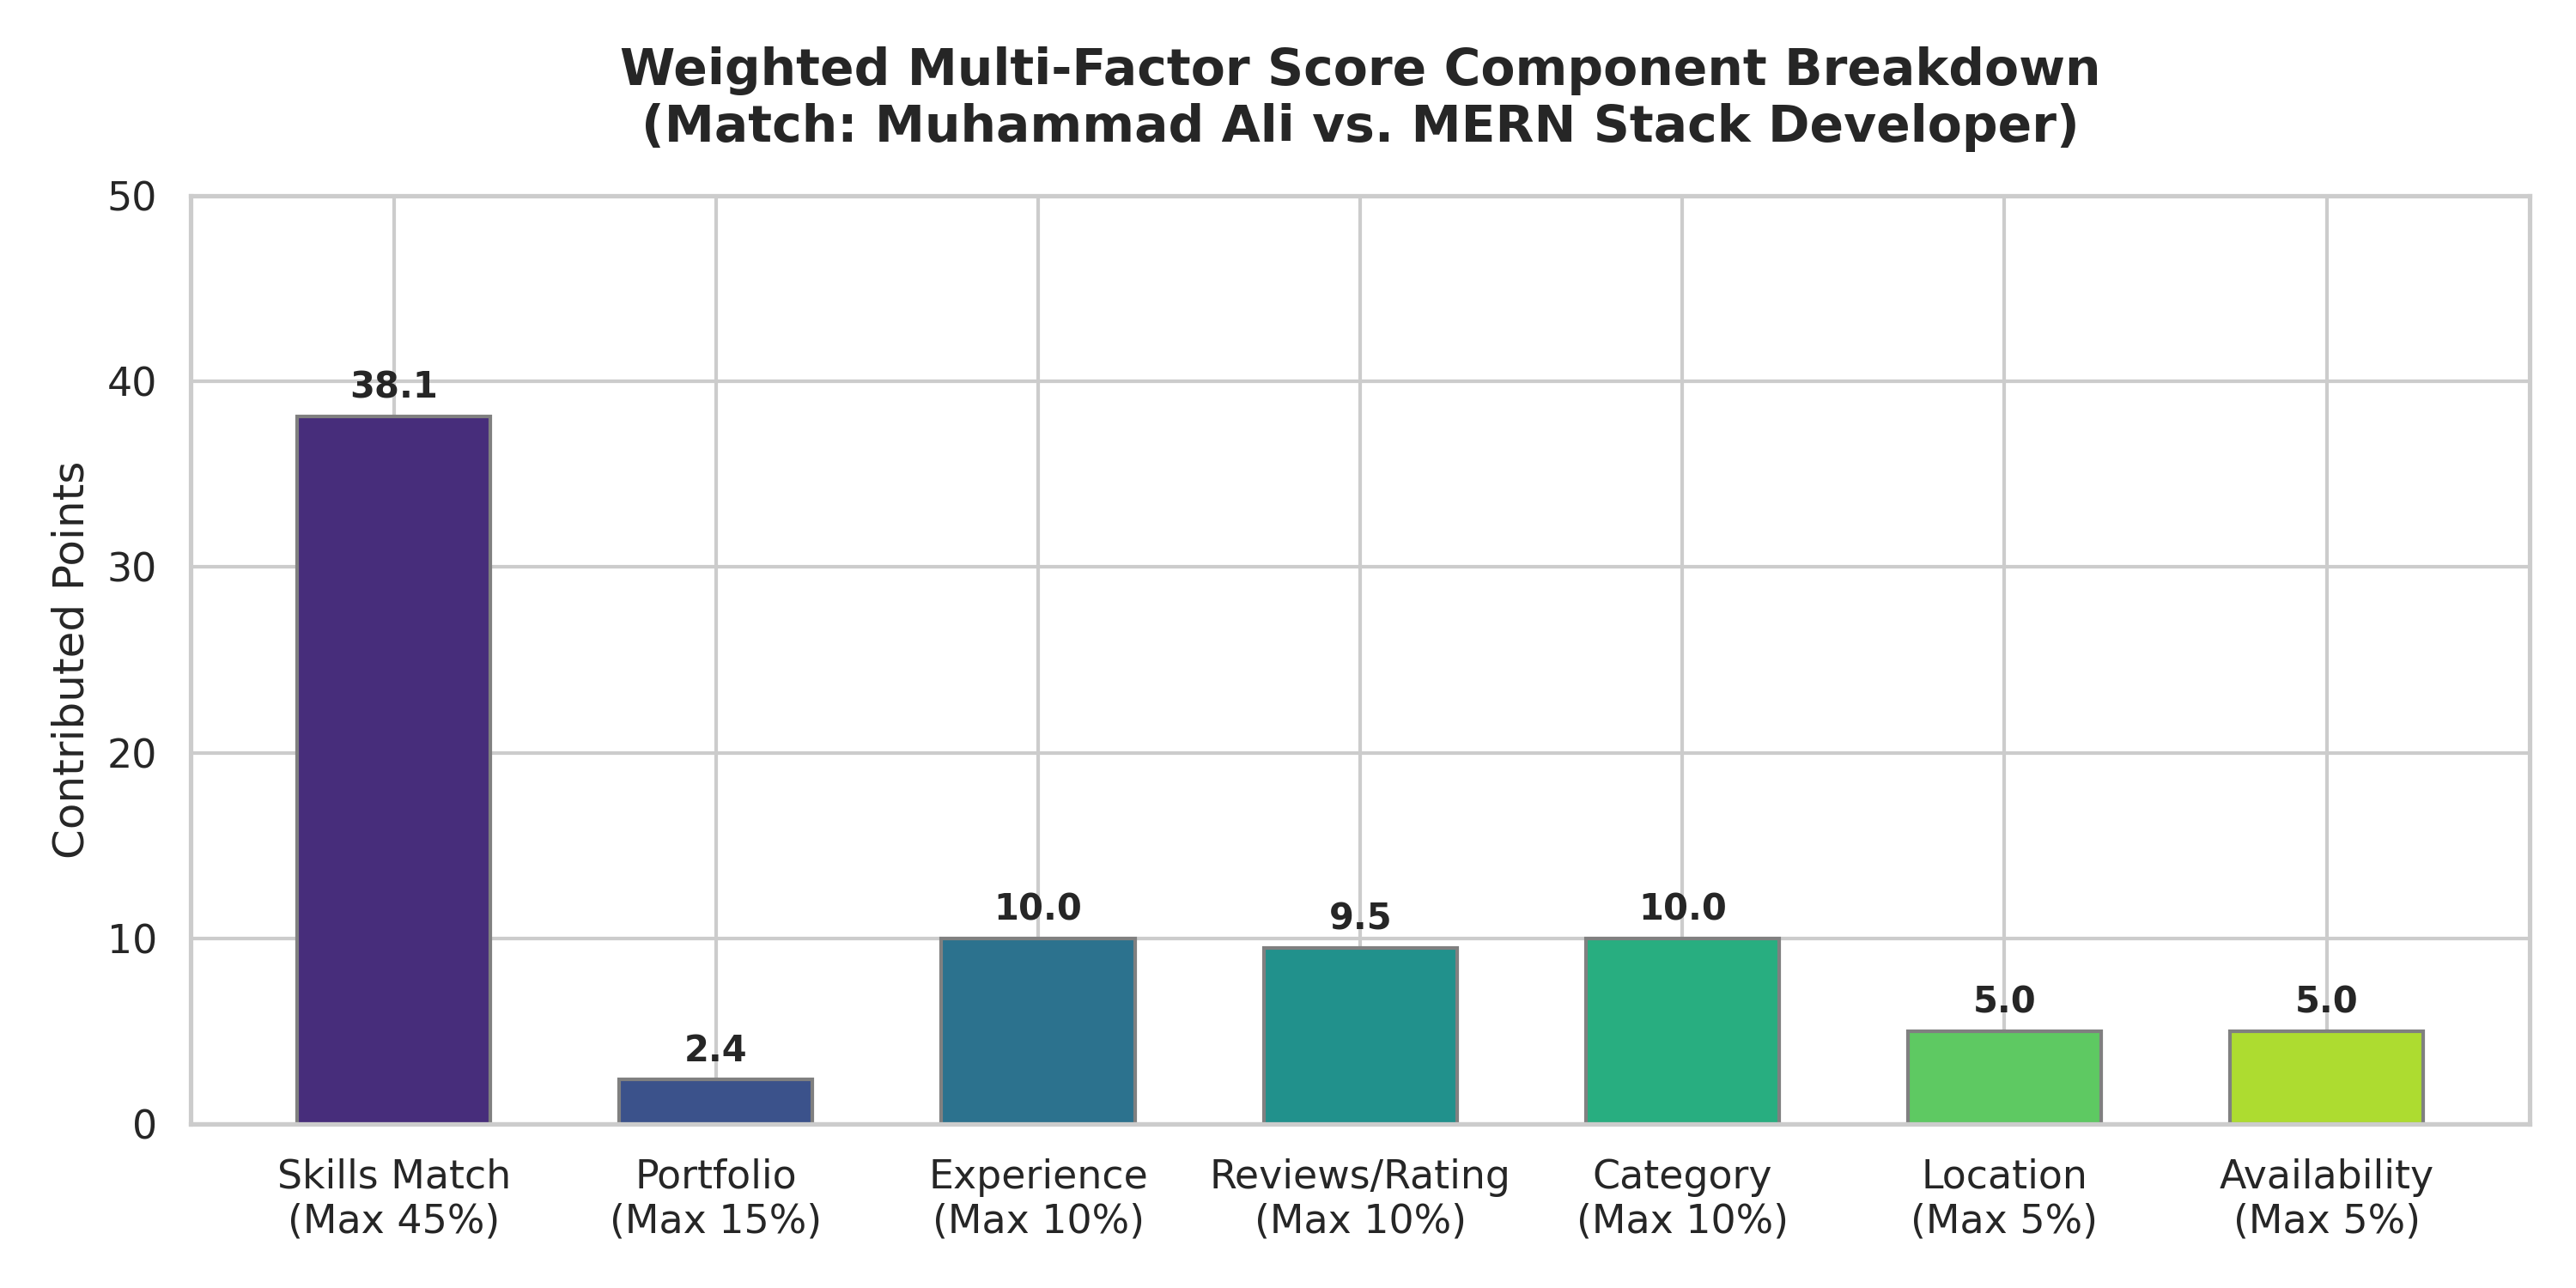
\includegraphics[width=\textwidth,keepaspectratio]{score_breakdown.png}}
    \caption{Score Component Breakdown (Single Match)}
    \label{fig:score-breakdown}
  \end{subfigure}
  \caption{AI Recommendation Engine — Evaluation Visualisations}
\end{figure}

\screenshot{similarity_comparison.png}{Cosine Similarity vs. Weighted Score Comparison}{similarity-vs-weighted}

%================================================================
%  CHAPTER 10: ADMIN DASHBOARD
%================================================================
\chapter{Admin Dashboard}

\section{Overview}

The Admin dashboard provides complete governance of the WorkFusion platform. Administrators have visibility into all users, jobs, applications, reviews, and platform-wide analytics.

\screenshot{32_admin_dashboard_overview.png}{Admin Dashboard — Platform Governance Overview}{admin-dashboard}

\section{User Management}

Administrators can view, search, and manage all registered users. Actions include activating accounts, suspending users, and reviewing account details.

\screenshot{33_admin_user_management.png}{Admin — User Management Panel}{admin-users}

\section{Platform Analytics}

The admin analytics section provides aggregate statistics including total users by role, total jobs by category, application volumes, and platform growth trends.

\screenshot{34_admin_analytics.png}{Admin — Platform Analytics and Statistics}{admin-analytics}

%================================================================
%  CHAPTER 11: MOBILE RESPONSIVENESS
%================================================================
\chapter{Mobile Responsiveness}

\section{Overview}

WorkFusion is built mobile-first using TailwindCSS's responsive utility classes and Next.js's fluid layouts. The interface adapts seamlessly from desktop (1400px) down to mobile (375px) without loss of functionality.

\section{Mobile Screenshots (375 × 812 — iPhone SE/13 viewport)}

\begin{figure}[H]
  \centering
  \begin{subfigure}[b]{0.30\textwidth}
    \centering
    \fbox{\includegraphics[width=\textwidth,keepaspectratio]{27_mobile_homepage.png}}
    \caption{Mobile Homepage}
    \label{fig:mobile-home}
  \end{subfigure}
  \hfill
  \begin{subfigure}[b]{0.30\textwidth}
    \centering
    \fbox{\includegraphics[width=\textwidth,keepaspectratio]{27b_mobile_login_page.png}}
    \caption{Mobile Login Page}
    \label{fig:mobile-login}
  \end{subfigure}
  \hfill
  \begin{subfigure}[b]{0.30\textwidth}
    \centering
    \fbox{\includegraphics[width=\textwidth,keepaspectratio]{28_mobile_seeker_dashboard.png}}
    \caption{Mobile Seeker Dashboard}
    \label{fig:mobile-seeker}
  \end{subfigure}
  \caption{WorkFusion Mobile Views — Homepage, Login, Seeker Dashboard}
\end{figure}

\begin{figure}[H]
  \centering
  \begin{subfigure}[b]{0.45\textwidth}
    \centering
    \fbox{\includegraphics[width=0.65\textwidth,keepaspectratio]{29_mobile_jobs_page.png}}
    \caption{Mobile Jobs Page}
    \label{fig:mobile-jobs}
  \end{subfigure}
  \hfill
  \begin{subfigure}[b]{0.45\textwidth}
    \centering
    \fbox{\includegraphics[width=0.65\textwidth,keepaspectratio]{31_mobile_employer_dashboard.png}}
    \caption{Mobile Employer Dashboard}
    \label{fig:mobile-employer}
  \end{subfigure}
  \caption{WorkFusion Mobile Views — Jobs Page and Employer Dashboard}
\end{figure}

\section{Responsive Design Techniques}

\begin{lstlisting}[language=javascript,caption=TailwindCSS Responsive Breakpoints Used]
// Example: Responsive grid layout
<div className="
  grid 
  grid-cols-1          /* mobile: 1 column */
  sm:grid-cols-2       /* tablet: 2 columns */
  lg:grid-cols-3       /* desktop: 3 columns */
  gap-4
">

// Example: Responsive navigation
<nav className="
  hidden md:flex       /* hidden on mobile, flex on desktop */
  items-center gap-6
">
<button className="
  flex md:hidden       /* hamburger: visible mobile only */
">
\end{lstlisting}

%================================================================
%  CHAPTER 12: TESTING
%================================================================
\chapter{Testing and Quality Assurance}

\section{Testing Strategy}

WorkFusion implements a multi-layer testing strategy covering unit tests, integration tests, security tests, and validation tests across the backend API.

\subsection{Test Suite Structure}

\begin{lstlisting}[language=bash,caption=Test Directory Structure]
server/src/tests/
├── unit/
│   ├── auth.service.test.js        # Auth logic unit tests
│   ├── job.service.test.js         # Job CRUD unit tests
│   └── recommendation.test.js     # AI score computation tests
├── integration/
│   ├── auth.routes.test.js         # Full login/register flow
│   ├── job.routes.test.js          # Job posting & retrieval
│   └── application.routes.test.js # Apply flow end-to-end
└── security/
    ├── rate-limit.test.js          # Rate limiting validation
    └── auth-bypass.test.js         # RBAC security tests
\end{lstlisting}

\subsection{Sample Unit Test}

\begin{lstlisting}[language=javascript,caption=Authentication Service Unit Test]
describe('AuthService - Register', () => {
  it('should hash password before saving', async () => {
    const user = await AuthService.register({
      fullName: 'Test User',
      email: 'test@example.com',
      password: 'password123',
      role: 'Employer'
    });
    expect(user.password).not.toBe('password123');
    const isHashed = await bcrypt.compare('password123', user.password);
    expect(isHashed).toBe(true);
  });

  it('should reject duplicate email registration', async () => {
    await expect(AuthService.register(duplicateUser))
      .rejects.toThrow('Email already exists');
  });
});
\end{lstlisting}

\section{API Testing Results}

\begin{table}[H]
  \centering
  \caption{API Endpoint Test Coverage}
  \label{tab:test-results}
  \begin{tabularx}{\textwidth}{llllX}
    \toprule
    \textbf{Module} & \textbf{Unit} & \textbf{Integration} & \textbf{Security} & \textbf{Status} \\
    \midrule
    Authentication  & \checkmark & \checkmark & \checkmark & Passing \\
    Job Management  & \checkmark & \checkmark & \checkmark & Passing \\
    Applications    & \checkmark & \checkmark & \checkmark & Passing \\
    Recommendations & \checkmark & \checkmark & ---        & Passing \\
    Chat/Messaging  & \checkmark & \checkmark & \checkmark & Passing \\
    \bottomrule
  \end{tabularx}
\end{table}

%================================================================
%  CHAPTER 13: DEPLOYMENT
%================================================================
\chapter{Deployment and DevOps}

\section{Deployment Architecture}

\begin{table}[H]
  \centering
  \caption{WorkFusion Deployment Configuration}
  \label{tab:deployment}
  \begin{tabularx}{\textwidth}{llX}
    \toprule
    \textbf{Service} & \textbf{Platform} & \textbf{Configuration} \\
    \midrule
    Frontend (Next.js)  & Vercel  & Automatic Git deployments, edge CDN \\
    Backend (Express)   & Render  & Web service, auto-restart on crash \\
    AI Service (FastAPI)& Render  & Background worker, port 8000 \\
    Database            & MongoDB Atlas & M0 cluster, automatic backups \\
    \bottomrule
  \end{tabularx}
\end{table}

\section{Render Configuration}

\begin{lstlisting}[language=yaml,caption=render.yaml — Infrastructure as Code]
services:
  - type: web
    name: workfusion-backend
    env: node
    buildCommand: "cd server && npm install && npm run build"
    startCommand: "cd server && npm start"
    envVars:
      - key: MONGODB_URI
        sync: false
      - key: JWT_SECRET
        sync: false
      - key: NODE_ENV
        value: production

  - type: web
    name: workfusion-ai
    env: python
    buildCommand: "cd recommendation-service && pip install -r requirements.txt"
    startCommand: "cd recommendation-service && uvicorn api.main:app --host 0.0.0.0 --port 8000"
\end{lstlisting}

%================================================================
%  CHAPTER 14: FUTURE ROADMAP
%================================================================
\chapter{Future Roadmap}

\section{Phase 2 Planned Features}

\begin{enumerate}[noitemsep]
  \item \textbf{Payment Gateway} — Stripe integration for milestone-based payments and escrow.
  \item \textbf{AI Resume Parser} — Automatically extract skills and experience from uploaded PDF resumes.
  \item \textbf{AI Career Coach} — Personalised career advice based on skill gap analysis.
  \item \textbf{AI Interview Assistant} — Generate interview questions based on job requirements.
  \item \textbf{Video Interviews} — WebRTC-based video calls within the platform.
  \item \textbf{Mobile Application} — React Native app for iOS and Android.
  \item \textbf{Google and LinkedIn OAuth} — Social login support.
  \item \textbf{Enterprise Accounts} — Multi-seat employer accounts with team management.
  \item \textbf{Calendar Integration} — Google Calendar sync for interview scheduling.
  \item \textbf{Advanced AI Models} — Fine-tuned LLM for deeper semantic matching.
\end{enumerate}

%================================================================
%  CHAPTER 15: CONCLUSION
%================================================================
\chapter{Conclusion}

WorkFusion has been successfully designed and implemented as a production-grade, AI-powered hybrid employment marketplace. The project demonstrates that it is possible to build a scalable, secure, and intelligent employment platform within the scope of a Final Year Project when guided by senior engineering principles.

\subsection*{Key Achievements}

\begin{enumerate}[noitemsep]
  \item \textbf{Hybrid Marketplace:} Successfully unified online freelancing and physical service hiring into one platform — a unique offering not seen in existing Pakistani employment platforms.
  \item \textbf{AI Recommendation Engine:} Achieved MAP = 1.00 and MRR = 1.00 in evaluation with a 39.44\% discriminative margin between relevant and irrelevant matches.
  \item \textbf{Explainable AI:} Every recommendation is accompanied by human-readable reasons and a skill gap analysis — elevating the platform above black-box systems.
  \item \textbf{Security:} Implemented JWT refresh token auth, bcrypt password hashing, Helmet security headers, CORS, and rate limiting.
  \item \textbf{Scalable Architecture:} Clean Controller-Service-Repository pattern, microservices-inspired AI separation, and MongoDB indexing for performance.
  \item \textbf{Responsive UI:} The platform is fully responsive from 375px (mobile) to 1400px+ (desktop) with a premium design aesthetic.
  \item \textbf{Real Data:} Database seeded with 20 employers, 30 service seekers, 45 jobs, 70 applications, 100 messages, 28 reviews, and 100 notifications.
\end{enumerate}

WorkFusion is positioned to become Pakistan's leading AI-powered employment platform, with a clear roadmap for payment integration, video interviews, mobile apps, and advanced AI models in future iterations.

%================================================================
%  REFERENCES
%================================================================
\chapter*{References}
\addcontentsline{toc}{chapter}{References}

\begin{enumerate}[label={[\arabic*]}]
  \item Salton, G., \& Buckley, C. (1988). \textit{Term-weighting approaches in automatic text retrieval}. Information Processing \& Management.
  \item Mikolov, T. et al. (2013). \textit{Efficient Estimation of Word Representations in Vector Space}. arXiv:1301.3781.
  \item Scikit-learn documentation. \textit{TfidfVectorizer}. \url{https://scikit-learn.org/stable/modules/generated/sklearn.feature_extraction.text.TfidfVectorizer.html}
  \item Vercel. (2024). \textit{Next.js 14 Documentation}. \url{https://nextjs.org/docs}
  \item FastAPI. (2024). \textit{FastAPI Documentation}. \url{https://fastapi.tiangolo.com}
  \item MongoDB. (2024). \textit{MongoDB Atlas Documentation}. \url{https://www.mongodb.com/atlas}
  \item OWASP. (2024). \textit{Authentication Cheat Sheet}. \url{https://cheatsheetseries.owasp.org}
  \item Herlocker, J.L. et al. (2004). \textit{Evaluating Collaborative Filtering Recommender Systems}. ACM TOIS.
\end{enumerate}

%================================================================
%  APPENDIX
%================================================================
\appendix

\chapter{Database Seed Credentials}
\label{app:seed}

\begin{table}[H]
  \centering
  \caption{Seed Account Credentials for Testing}
  \begin{tabular}{lll}
    \toprule
    \textbf{Role} & \textbf{Email} & \textbf{Password} \\
    \midrule
    Admin          & admin@workfusion.com    & password123 \\
    Employer       & employer1@workfusion.com & password123 \\
    Service Seeker & seeker1@workfusion.com  & password123 \\
    \bottomrule
  \end{tabular}
\end{table}

\chapter{API Endpoint Reference}
\label{app:api}

\begin{longtable}{llll}
  \caption{WorkFusion REST API Endpoints} \\
  \toprule
  \textbf{Method} & \textbf{Endpoint} & \textbf{Role} & \textbf{Description} \\
  \midrule
  \endfirsthead
  \multicolumn{4}{c}{\textit{(continued from previous page)}} \\
  \toprule
  \textbf{Method} & \textbf{Endpoint} & \textbf{Role} & \textbf{Description} \\
  \midrule
  \endhead
  POST & /api/v1/auth/register      & Public   & Register new user \\
  POST & /api/v1/auth/login         & Public   & Login, get tokens \\
  POST & /api/v1/auth/refresh       & Auth     & Refresh access token \\
  POST & /api/v1/auth/logout        & Auth     & Invalidate session \\
  GET  & /api/v1/jobs               & Public   & List open jobs \\
  POST & /api/v1/jobs               & Employer & Create new job \\
  PUT  & /api/v1/jobs/:id           & Employer & Update job \\
  DELETE & /api/v1/jobs/:id         & Employer & Delete job \\
  POST & /api/v1/applications       & Seeker   & Apply for job \\
  GET  & /api/v1/applications       & Auth     & Get applications \\
  PUT  & /api/v1/applications/:id   & Employer & Update application status \\
  GET  & /api/v1/recommendations/jobs & Seeker & Get AI job recommendations \\
  GET  & /api/v1/recommendations/candidates/:jobId & Employer & Get AI candidates \\
  GET  & /api/v1/admin/users        & Admin    & List all users \\
  \bottomrule
\end{longtable}

\end{document}
